\subsection{Infraestructura y herramientas}
\subsubsection{Descripción general de la infraestructura}
La infraestructura y las herramientas son la base sobre la que se construirán
los diferentes proyectos de aprendizaje automático. Se encargan de proporcionar
un entorno de desarrollo e investigación eficiente, que permita a los miembros
del equipo centrarse en el desarrollo de modelos sin tener que preocuparse por
la configuración. Concretamente, se han desplegado dos plataformas 
que vienen a cubrir varias de las necesidades fundamentales de los proyectos
como son la gestión y exploración de datasets, la monitorización de experimentos o
el almacenamiento de modelos de inteligencia artificial. Además, se ha añadido un sistema de autenticación 
para garantizar la seguridad y privacidad de los datos.\medskip

Esta infraestructura se ha desplegado en un servidor interno de la empresa
utilizando contenedores de Docker. La elección de esta tecnología se debe a
que permite la creación de entornos aislados y portables, lo que facilita el
despliegue de las aplicaciones. Se ha utilizado Docker Compose para
sincronizar el despliegue de los diferentes servicios, lo que permite
realizar despliegues automatizados mediante las acciones de GitLab CI. La
figura \ref{fig:internal-server} muestra una vista general de la infraestructura
desplegada en el servidor interno de la empresa, donde se pueden observar
como se integran los diferentes servicios y sus respectivas conexiones. Además,
se puede observar que todos los servicios están interconectados mediante un
proxy inverso mediante Nginx, que se encarga de redirigir las peticiones en 
función de la URL. Esto permite que todos los servicios sean
accesibles desde el exterior a través de un único punto de entrada y que el
sistema de autenticación sea común para todos ellos.

\begin{figure}[ht]
    \centering
    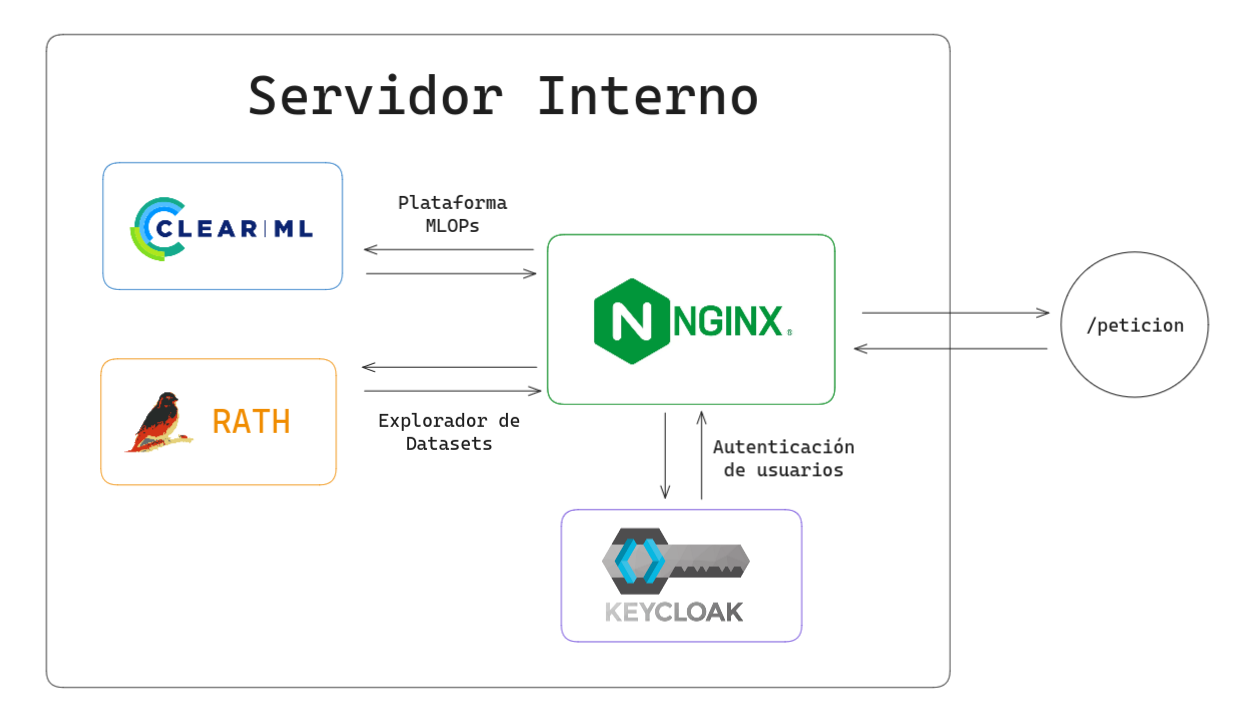
\includegraphics[width=\textwidth]{internal-server.png}
    \caption{Vista general del proyecto}\label{fig:internal-server}
\end{figure}

\subsubsection{Plataformas integradas}
Previo a la elección de las plataformas integradas, se realizó una evaluación
a nivel de equipo para determinar las necesidades que se debían cubrir. Se
identificaron las siguientes funcionalidades fundamentales:

\begin{itemize}
    \item F1: Versionado y almacenamiento de dataset.
    \item F2: Monitorización de experimentos.
    \item F3: Almacenamiento de modelos de inteligencia artificial.
    \item F4: Integración de métricas en datasets y visualización de resultados.
    \item F5: Exploración de datasets.
\end{itemize}

Una vez identificadas las necesidades, se consensuó un criterio de selección
para las plataformas integradas. Este criterio es un criterio de mínimos, es
decir, se seleccionarán las plataformas que cumplan con el criterio mínimo
establecido y que, además, ofrezcan funcionalidades adicionales que puedan
ser de utilidad para el equipo. El criterio de selección se basa en los
siguientes aspectos: 

\begin{itemize}
    \item \textbf{C1 (Facilidad de uso):} Se valora muy positivamente la facilidad de uso de las
    plataformas, ya que se considera que no todo el equipo no tiene experiencia
    previa en el uso de estas herramientas.
    \item \textbf{C2 (Integración con otras herramientas):} Es fundamental que las
    plataformas integradas sean compatibles con las librerías y herramientas
    que se utilizan generalmente en proyectos (TensorFlow, PyTorch, etc.).
    \item \textbf{C3 (Poca dependencia sobre la infraestructura):} Medimos la dependencia
    sobre una plataforma como el numero de acciones que se deben realizar para
    migrar un proyecto vanilla, es decir, un proyecto que no ha sido
    desarrollado con la plataforma en mente. Y penalizando aquellas practicas
    que sean propias de la plataforma y que no sean comunes en la industria.
\end{itemize}

Con estos criterios en mente, se tuvieron en cuenta las siguientes
plataformas a la hora de realizar la evaluación: MLflow, ClearML, Kedro, ZenML, Data Version Controller (DVC),
Rath, Apache Superset. Cada una de estas plataformas tiene diferentes enfoques y 
funcionalidades, pero todas ellas cubren una o varias de las necesidades fundamentales
identificadas, por lo que se consideraron candidatas para su integración en la
infraestructura. La infraestructura final se compondrá de una o varias de estas
plataformas en función de los criterios previamente establecidos. A continuación, se 
muestra un análisis detallado de las plataformas evaluadas y las funcionalidades que ofrecen.

\begin{itemize}
    \item \textbf{MLflow:} MLflow es una plataforma MLOPs de código abierto para la gestión del ciclo de vida de
    los modelos. Ofrece una interfaz de usuario para el seguimiento de experimentos, la gestión de modelos 
    y la implementación de modelos en diferentes entornos. MLflow es compatible con la mayor parte de librerías de aprendizaje 
    automático, como TensorFlow o PyTorch. Uno de los puntos fuertes de MLflow es su gran comunidad, ya que es
    una de las plataformas más utilizadas en la industria. Sin embargo, no ofrece funcionalidades relacionadas con
    la gestión, evaluación o versionado de datasets ni con la exploración de los mismos. La dependencia sobre la
    plataforma varía en función de la tarea que se quiera realizar, pero en general, es una plataforma que no
    ata al usuario a su ella. La documentación se queda corta en cuestión de claridad y ejemplos, lo que puede
    dificultar la adopción de la plataforma por parte de los miembros del equipo.
    \item \textbf{ClearML:} ClearML al igual que MLflow, es una plataforma MLOps de código abierto que ofrece
    las mismas funcionalidades que MLflow en relación a la gestión a la gestión de experimentos, pero con la
    diferencias, que este si cuenta con funcionalidades relacionadas con la gestión, evaluación o versionado de
    datasets. ClearML también es compatible con la mayor parte de librerías populares aunque no tantas ni tan
    variadas como MLflow, pero ofrece una API que permite de la integración de estas de forma manual. La
    dependencia sobre la plataforma es mínima, ya que con pocos cambios se pueden lanzar experimentos sobre
    un código base. La documentación es clara y ofrece ejemplos en formato tanto de texto como de video, con
    proyectos sencillos y claros que permiten entender rápidamente el funcionamiento de la plataforma. El 
    principal punto débil de ClearML es que no cuenta con una gran comunidad, lo que puede dificultar a
    la hora de encontrar soluciones a ciertas problemáticas. Otro de sus puntos débiles es que por defecto
    no cuenta con un sistema de autenticación robusto, lo que te obliga a implementar uno por tu cuenta.
    \item \textbf{Data Version Controller (DVC):} DVC y DVC Studio son dos herramientas de código abierto que
    están diseñadas para manejar grandes volúmenes de datos, modelos y experimentos. DVC
    se centra en el versionado y almacenamiento de datasets, mientras que DVC Studio se centra en la
    monitorización de experimentos, visualización de resultados y almacenamiento de modelos. Además, 
    DVC Live proporciona integraciones con un número considerable de librerías de aprendizaje automático.
    La documentación está bien estructurada aunque no es tan clara como la de ClearML, pero cuenta con una
    comunidad bastante activa. En cuanto a los aspectos negativos de DVC, la principal desventaja es que
    la curva de aprendizaje es bastante pronunciada, lo que dificulta su adopción. Otro punto en contra
    es la dependencia gigantesca que tienen los proyectos que usan DVC, ya que se necesita de muchos archivos
    de configuración, integraciones manuales dentro del código y un dominio completo de los comandos de la
    herramienta para poder trabajar con ella.
    \item \textbf{Kedro:} TODO:
    \item \textbf{ZenML:} TODO:
    \item \textbf{Rath:} TODO:
    \item \textbf{Apache Superset:} TODO:
    \item \textbf{Grafana:} TODO:
\end{itemize}

Para finalizar con la evaluación, se ha realizado una tabla comparativa que muestra
las funcionalidades y criterios que cumple cada una de ellas de forma resumida.
\begin{table}[ht]
    \centering 
    \begin{tabular}{lccccccccc}  
        
        \toprule
        \multirow{2}{*}{\parbox[c]{.2\linewidth}{\centering Tecnología}} & 
        \multicolumn{5}{c}{\textbf{Funcionalidades}} && 
        \multicolumn{3}{c}{\textbf{Criterios}} \\ 
        
        \cmidrule{2-6} \cmidrule{8-10}
        & {\centering F1} & {F2} & {F3}& {F4} & {F5} && {C1} & {C2} & {C3}\\
        
        \midrule
        MLflow           & --     & \check & \check & --     & --     && \check & \check & \check \\
        ClearML          & \check & \check & \check & \check & --     && \check & \check & \check \\
        DVC              & \check & \check & \check & \check & --     && --     & \check & --     \\ 
        Kedro            & --     & --     & --     & --     & --     && --     & --     & --     \\  
        ZenML            & --     & --     & --     & --     & --     && --     & --     & --     \\ 
        Rath             & --     & --     & --     & --     & \check && \check & --     & \check \\ 
        Apache Superset  & \check & --     & --     & \check & --     && --     & --     & \check \\ 
        Grafana          & \check & --     & --     & \check & --     && --     & --     & \check \\ 
        \bottomrule
        
    \end{tabular}
    \caption{Tabla comparativa de las plataformas evaluadas}
    \label{tab:comparative-table} 
\end{table}


\subsubsection{Herramientas de desarrollo}
\subsubsection{Seguridad y priviacidad}
\subsubsection{Despligue Automatizado}